% !TeX root =  main.tex

\hypertarget{solving-polynomial-equations-by-factoring}{%
\section{Solving by
Factoring}\label{solving-by-factoring}}

\hypertarget{properties-of-equations}{%
\subsection{Properties of Equations}\label{properties-of-equations}}

Two equations are said to be
\textbf{\emph{equivalent}} if and only if they have the same solution
set.

\noindent
\textbf{\MakeUppercase{Transforms that can be used to solve an equation}:}

\begin{itemize}
\item
  \textbf{Adding or subtracting} the same quantity to both sides of an equation.
  For example, \(x-1=2\) is equivalent to \(x-1+1=2+1\).
\item
  \textbf{Multiplying or dividing} both sides of an equation \textbf{by a
  non-zero quantity}. For example \(2x=4\) is equivalent to
  \(\frac{2x}{2}=\frac{4}{2}\).
  
  Note that multiplying an expression to both sides may create solutions which are not solutions of the original equation. Such a solution is called an \textbf{\emph{extraneous solutions}}.
\item
  \textbf{Applying an identity} to transform one side of the equation. For
  example, \(x^2-1=0\) is equivalent to \((x-1)(x+1)=0\), where the
  identity \(x^2-1=(x-1)(x+1)\) was applied.

\item \textbf{Applying a function} to both sides of the equation. For example, taking square of both sides of the equation $\sqrt{x}=2$ yields a new equation $x=4$. In general, solutions of the resulting equation include solution(s) of the original equation and may also have extraneous solutions. For example, taking squares of both sides of the equation \(x=1\) produces the equation \(x^2=1\). The
new equation \(x^2=1\) has two solutions \(x=-1\) and \(x=1\), but the
original equation \(x=1\) only has one solution. The solution \(x=-1\)
of the equation \(x^2=1\) is an extraneous solution of the equation
\(x=1\).
\end{itemize}


\hypertarget{quadratic-equations}{%
\subsection{Quadratic Equations}\label{quadratic-equations}}

A \textbf{polynomial equation} is an equation that can be written in the
form \[
a_{n}x^{n}+a_{n-1}x^{n-1}+\cdots+a_{2}x^{2}+a_{1}x+a_{0}=0,
\] where \(n\) is a positive integer and \(a_n\ne 0\).

A polynomial equation is called a \textbf{\emph{quadratic equation}} if
\(n=2\). For example, \(2x^2+5x-3=0\). We often write a quadratic
equation in its \textbf{\emph{standard form}} \[a x^2+bx+c=0,\] where
\(a\), \(b\) and \(c\) are numbers, and \(a\neq 0\).

The \textbf{\emph{Zero-product
property}}:
\[A\cdot B=0 \quad ~~\text{if and only if}~~  \quad A=0 ~~\text{or}~~ B=0,\]


\begin{example}
Solve the equation \[2x^2+5x=3.\]
\end{example}
\vspace*{5\baselineskip}

\begin{example}
Solve the equation \[(x-2)(x+3)=-4.\]
\end{example}
\vspace*{5\baselineskip}

\begin{example}
A rectangular garden is surrounded by a path of uniform width. If the
dimension of the garden is \(10\) meters by \(16\) meters and the total
area is 216 square meters, determine the width of the path.

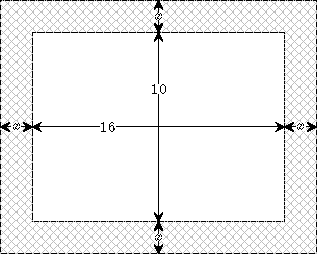
\includegraphics{figs/tikz-rectangular-uniform-width.png}\\
\end{example}
\vspace*{5\baselineskip}

\newpage

\subsection{Practice}

\begin{exercise}
Solve the equation by factoring.

\begin{enumerate}

\item
  \(x^2-3x+2=0\)
\item
  \(2x^2-3x=5\)
\item
  \((x-1)(x+3)=5\)
\item
  \(\frac13(2-x)(x+5)=4\)
\end{enumerate}
\end{exercise}

\begin{exercise}
Find all real solutions of the equation by factoring.

\begin{enumerate}

\item
  \(4(x-2)^2-9=0\)
\item
  \(2x^3-18x=0\)
\item
  \(3x^4-2x^2=1\)
\item
  \(x^3-3x^2-4x+12=0\)
\end{enumerate}
\end{exercise}

\begin{exercise}
A paint measuring \(3\) inches by \(4\) inches is surrounded by a frame
of uniform width. If the combined area of the paint and the frame is
\(30\) square inches, determine the width of the frame.


\includegraphics{figs/tikz-paint-uniform-width.png}\\
\end{exercise}
\vspace*{5\baselineskip}

\begin{exercise}
A rectangle whose length is \(2\) meters longer than its width has an
area \(8\) square meters. Find the width and the length of the
rectangle.
\end{exercise}
\vspace*{5\baselineskip}

\begin{exercise}
The product of two \textbf{consecutive negative odd} numbers is \(35\).
Find the numbers.
\end{exercise}
\vspace*{5\baselineskip}

\begin{exercise}
In a right triangle, the long leg is 2 inches more than double of the
short leg. The hypotenuse of the triangle is 1 inch longer than the long
leg. Find the length of the shortest side.
\end{exercise}
\vspace*{5\baselineskip}

\begin{exercise}
A ball is thrown upwards from a rooftop. It will reach a maximum
vertical height and then fall back to the ground. The height \(h(t)\) of
the ball from the ground after time \(t\) seconds is
\(h(t)=-16t^2 + 48t + 160\) feet. How long it will take the ball to hit
the ground?
\end{exercise}

\vspace*{5\baselineskip}
\begin{exercise}
A toy factory estimates that the demand of a particular toy is
\(300 -x\) units each week if the price is \$\(x\) dollars per unit.
% Each week there is a fixed cost \$40,000 to produce the demanded toys.
% The weekly revenue is a function of the price given by \(R(x)=x(30-x)\)

\begin{enumerate}

\item
  Find the function that models the weekly revenue, \(R\), received when
  the selling price is \$\(x\) per unit.
\item
  What the price range so the revenue is nonnegative.
\end{enumerate}
\end{exercise}

